\documentclass[11pt]{article}

% --- PACKAGES ---
\usepackage{amsmath}
\usepackage{amssymb}
\usepackage{graphicx}
\usepackage{tikz}
\usepackage{pgfplots}
\usepackage{float}
\usepackage{subcaption}
\usepackage{geometry}
\usepackage{enumerate}
\usepackage{enumitem}

% --- SETTINGS ---
\geometry{a4paper, margin=1in}
\pgfplotsset{compat=1.18}
\usetikzlibrary{patterns,decorations.pathreplacing}

% --- COMMANDS ---
\newcommand{\dd}{\mathrm{d}}

% --- DOCUMENT ---\\


% Define example environment
\newenvironment{example}[1]{
    \begin{trivlist}
    \item[\textbf{Example:}] #1
    \vspace{0.5em}
}{
    \end{trivlist}
    \vspace{1em}
}

\begin{document}
	% Reset figure counter for this lecture
	\renewcommand{\thefigure}{7.\arabic{figure}}
	
	% --- TITLE BLOCK ---
	\thispagestyle{empty}
	\noindent
	\begin{tabular*}{\textwidth}{l @{\extracolsep{\fill}} r}
		\textbf{Signals and Systems} & \textbf{Lecture 7 Examples} \\
		\textit{Ahmed Rabei} & \textit{Fall 2025} \\
	\end{tabular*}
	\hrule
	\vspace{0.4cm}
	\begin{center}
		\Large\textbf{Lecture 7 Examples: Continuous-Time Fourier Series}
	\end{center}
	\vspace{0.4cm}

\begin{example}[1. Fourier Series Coefficients for a Periodic Signal]
\textbf{Problem:}
Find the Fourier series coefficients $a_k$ for:
$$x(t) = \begin{cases}
    1 & \text{for } 0 \leq t < \pi \\
    -1 & \text{for } \pi \leq t < 2\pi
\end{cases}$$
with period $T_0 = 2\pi$ and fundamental frequency $\omega_0 = 1$.

\begin{figure}[H]
    \centering
    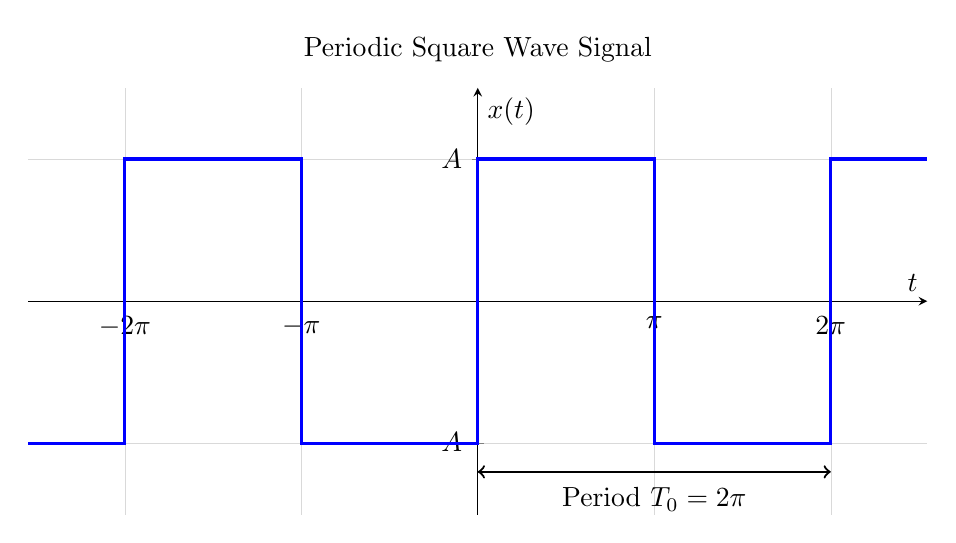
\begin{tikzpicture}
	\begin{axis}[
		width=13cm,
		height=7cm,
		axis lines=middle,
		xlabel={$t$},
		ylabel={$x(t)$},
		title={Periodic Square Wave Signal},
		xmin=-8, xmax=8,
		ymin=-1.5, ymax=1.5,
		xtick={-6.28, -3.14, 3.14, 6.28},
		xticklabels={$-2\pi$, $-\pi$, $\pi$, $2\pi$},
		ytick={-1, 1},
		yticklabels={$-A$, $A$},
		grid=major,
		grid style={line width=.1pt, draw=gray!30},
		no marks,
		]
		
		% Use 'const plot' for a cleaner way to draw square waves
		\addplot[const plot, blue, very thick] coordinates {
			(-8, -1)
			(-6.283, 1)
			(-3.141, -1)
			(0, 1)
			(3.141, -1)
			(6.283, 1)
			(8, 1)
		};
		
		% Add a single, correct period marker
		\draw[<->, thick] (axis cs:0, -1.2) -- (axis cs:6.283, -1.2) node[midway, below=2pt] {Period $T_0 = 2\pi$};
		
	\end{axis}
\end{tikzpicture}
    \caption{The periodic square wave signal $x(t)$.}
    \label{fig:square_wave}
\end{figure}

\textbf{Solution:}

$$a_k = \frac{1}{T_0} \int_{T_0} x(t) e^{-jk\omega_0 t} \dd t = \frac{1}{2\pi} \int_{0}^{2\pi} x(t) e^{-jkt} \dd t$$

$$= \frac{1}{2\pi} \left[ \int_{0}^{\pi} e^{-jkt} \dd t - \int_{\pi}^{2\pi} e^{-jkt} \dd t \right]$$

For $k \neq 0$:
$$a_k = \frac{1}{2\pi jk} [2e^{-jk\pi} - 1 - e^{-j2k\pi}] = \frac{1}{\pi jk} [e^{-jk\pi} - 1]$$

Since $e^{-jk\pi} = (-1)^k$:
$$a_k = \frac{1}{\pi jk} [(-1)^k - 1]$$

\textbf{Answer:}
$$a_k = \begin{cases}
    0 & \text{for even } k \\
    \frac{-2j}{\pi k} & \text{for odd } k
\end{cases}$$
\end{example}

\vspace{0.5em}
\hrule
\vspace{0.5em}

\begin{example}[2. Fourier Series of a Sum of Sinusoids]
\textbf{Problem:}
Find the Fourier series representation of:
$$x(t) = 2\cos(3t) + \sin(5t)$$

\textbf{Solution:}

\textbf{Fundamental period:} $T_0 = 2\pi$, $\omega_0 = 1$

\textbf{Express as complex exponentials:}
$$x(t) = e^{j3\omega_0 t} + e^{-j3\omega_0 t} + \frac{1}{2j}e^{j5\omega_0 t} - \frac{1}{2j}e^{-j5\omega_0 t}$$

\textbf{Answer:}
$$a_k = \begin{cases}
    1 & \text{for } k = \pm 3 \\
    \mp \frac{j}{2} & \text{for } k = \pm 5 \\
    0 & \text{otherwise}
\end{cases}$$
\end{example}

\vspace{0.5em}
\hrule
\vspace{0.5em}

\begin{example}[3. Fourier Series of a Triangular Wave]
\textbf{Problem:}
Find the Fourier series coefficients for:
$$x(t) = \begin{cases}
    t & \text{for } 0 \leq t \leq 1 \\
    2-t & \text{for } 1 \leq t \leq 2
\end{cases}$$
with period $T_0 = 2$ and fundamental frequency $\omega_0 = \pi$.

\begin{figure}[H]
    \centering
    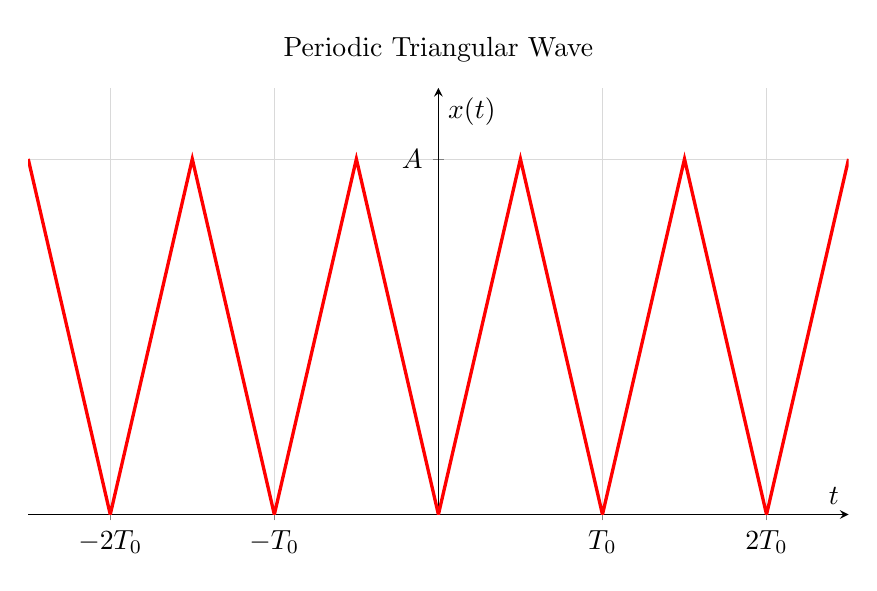
\begin{tikzpicture}
	\begin{axis}[
		width=12cm,
		height=7cm,
		axis lines=middle,
		xlabel={$t$},
		ylabel={$x(t)$},
		title={Periodic Triangular Wave},
		xmin=-5, xmax=5,
		ymin=0, ymax=1.2,
		xtick={-4, -2, 2, 4},
		xticklabels={$-2T_0$, $-T_0$, $T_0$, $2T_0$},
		ytick={1},
		yticklabels={$A$},
		grid=major,
		grid style={line width=.1pt, draw=gray!30},
		]
		
		% Plot the triangular wave
		\draw[red, very thick]
		(axis cs:-5,1) -- (axis cs:-4,0) -- (axis cs:-3,1) -- (axis cs:-2,0)
		-- (axis cs:-1,1) -- (axis cs:0,0) -- (axis cs:1,1) -- (axis cs:2,0)
		-- (axis cs:3,1) -- (axis cs:4,0) -- (axis cs:5,1);
		
		% Add a single, clear period label
		\draw[<->, thick] (axis cs:0, -0.15) -- (axis cs:2, -0.15) node[midway, below=2pt] {Period $T_0$};
		
	\end{axis}
\end{tikzpicture}
    \caption{The periodic triangular wave signal $x(t)$.}
    \label{fig:triangular_wave}
\end{figure}

\textbf{Solution:}

$$a_k = \frac{1}{T_0} \int_{T_0} x(t) e^{-jk\omega_0 t} \dd t = \frac{1}{2} \int_{0}^{2} x(t) e^{-jk\pi t} \dd t$$

After integration by parts:
$$a_k = \frac{\sin(k\pi)}{k\pi} + \frac{\cos(k\pi) - 1}{(k\pi)^2}$$

\textbf{Answer:}
$$a_k = \begin{cases}
    \frac{1}{2} & \text{for } k = 0 \\
    0 & \text{for even } k \neq 0 \\
    \frac{-2}{(k\pi)^2} & \text{for odd } k
\end{cases}$$
\end{example}

\vspace{0.5em}
\hrule
\vspace{0.5em}

\begin{example}[4. Fourier Series of $|\cos(t)|$]
\textbf{Problem:}
Find the Fourier series coefficients for $x(t) = |\cos(t)|$.

\begin{figure}[H]
    \centering
    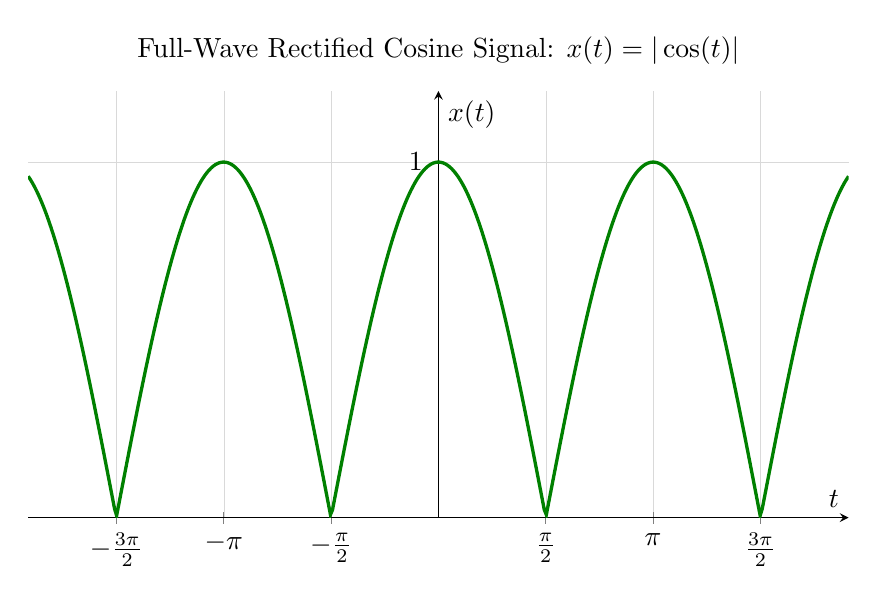
\begin{tikzpicture}
	\begin{axis}[
		width=12cm,
		height=7cm,
		axis lines=middle,
		xlabel={$t$},
		ylabel={$x(t)$},
		title={Full-Wave Rectified Cosine Signal: $x(t) = |\cos(t)|$},
		xmin=-6, xmax=6,
		ymin=0, ymax=1.2,
		xtick={-4.71, -3.14, -1.57, 0, 1.57, 3.14, 4.71},
		xticklabels={$-\frac{3\pi}{2}$, $-\pi$, $-\frac{\pi}{2}$, $0$, $\frac{\pi}{2}$, $\pi$, $\frac{3\pi}{2}$},
		ytick={1},
		yticklabels={$1$},
		grid=major,
		grid style={line width=.1pt, draw=gray!30},
		no marks,
		]
		
		% Plot the absolute value of cosine - multiple periods
		\addplot[green!50!black, very thick, domain=-6:6, samples=400] {abs(cos(deg(x)))};
		
		% Add period labels
		\draw[<->, thick] (axis cs:-3.14, -0.15) -- (axis cs:-1.57, -0.15) node[midway, below=2pt] {$T_0$};
		\draw[<->, thick] (axis cs:-1.57, -0.15) -- (axis cs:0, -0.15) node[midway, below=2pt] {$T_0$};
		\draw[<->, thick] (axis cs:0, -0.15) -- (axis cs:1.57, -0.15) node[midway, below=2pt] {$T_0$};
		\draw[<->, thick] (axis cs:1.57, -0.15) -- (axis cs:3.14, -0.15) node[midway, below=2pt] {$T_0$};
		
	\end{axis}
\end{tikzpicture}
    \caption{The signal $x(t) = |\cos(t)|$.}
    \label{fig:abs_cos}
\end{figure}

\textbf{Solution:}

\textbf{Period:} $T_0 = \pi$, $\omega_0 = 2$

For $|\cos(t)|$ over $[0, \pi]$:
$$|\cos(t)| = \begin{cases}
    \cos(t) & \text{for } 0 \leq t \leq \pi/2 \\
    -\cos(t) & \text{for } \pi/2 < t \leq \pi
\end{cases}$$

$$a_k = \frac{1}{T_0} \int_{T_0} |\cos(t)| e^{-jk\omega_0 t} \dd t = \frac{1}{\pi} \left[ \int_{0}^{\pi/2} \cos(t) e^{-j2kt} \dd t + \int_{\pi/2}^{\pi} (-\cos(t)) e^{-j2kt} \dd t \right]$$

After integration:
$$a_k = \frac{2}{\pi(1-4k^2)} \cos(k\pi)$$

\textbf{Answer:}
$$a_k = \begin{cases}
    \frac{2}{\pi} & \text{for } k = 0 \\
    \frac{2(-1)^k}{\pi(1-4k^2)} & \text{for } k \neq 0
\end{cases}$$
\end{example}

\vspace{0.5em}
\hrule
\vspace{0.5em}

\begin{example}[5. Fourier Series of a Shifted Periodic Square Wave]
\textbf{Problem:}
Find Fourier series coefficients for periodic square wave $y(t)$ with period $T_0$ and pulse width $2T_1$.

\begin{figure}[H]
    \centering
    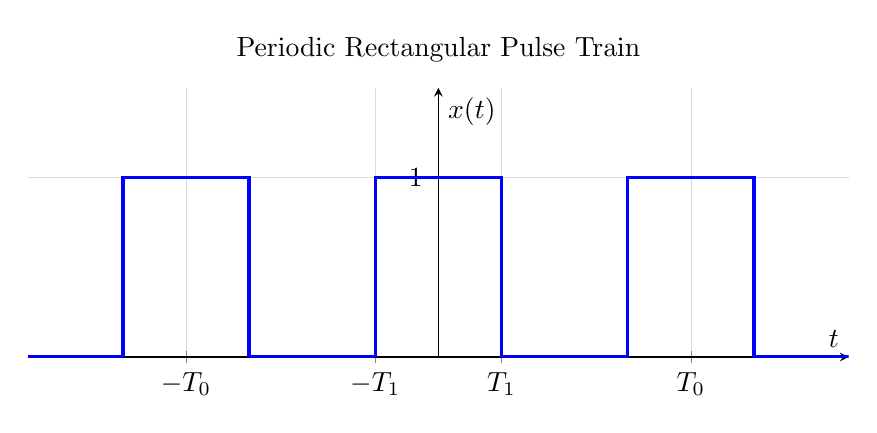
\begin{tikzpicture}
	\begin{axis}[
		width=12cm,
		height=5cm,
		title={Periodic Rectangular Pulse Train},
		xlabel={$t$},
		ylabel={$x(t)$},
		axis lines=middle,
		xmin=-6.5, xmax=6.5,
		ymin=0, ymax=1.5,
		xtick={-4, -1, 1, 4},
		xticklabels={$-T_0$, $-T_1$, $T_1$, $T_0$},
		ytick={1},
		grid=major,
		grid style={line width=.1pt, draw=gray!30},
		]
		
		% Draw the pulses (using representative values T0=4, T1=1)
		% Central Pulse
		\draw[blue, very thick] (axis cs:-1,0) -- (axis cs:-1,1) -- (axis cs:1,1) -- (axis cs:1,0);
		% Next Pulse
		\draw[blue, very thick] (axis cs:3,0) -- (axis cs:3,1) -- (axis cs:5,1) -- (axis cs:5,0);
		% Previous Pulse
		\draw[blue, very thick] (axis cs:-5,0) -- (axis cs:-5,1) -- (axis cs:-3,1) -- (axis cs:-3,0);
		% Zero lines connecting them
		\draw[blue, very thick] (axis cs:-6.5,0) -- (axis cs:-5,0);
		\draw[blue, very thick] (axis cs:-3,0) -- (axis cs:-1,0);
		\draw[blue, very thick] (axis cs:1,0) -- (axis cs:3,0);
		\draw[blue, very thick] (axis cs:5,0) -- (axis cs:6.5,0);
		
		% Add period marker
		\draw[<->, thick] (axis cs:0, -0.3) -- (axis cs:4, -0.3) node[midway, below=2pt] {Period $T_0$};
		
	\end{axis}
\end{tikzpicture}
    \caption{The periodic shifted square wave signal $y(t)$.}
\end{figure}

\textbf{Solution:}
$$a_k = \frac{1}{T_0} \int_{-T_1}^{T_1} e^{-jk\omega_0 t} \dd t = \frac{2T_1}{T_0} \text{sinc}\left(\frac{2k T_1}{T_0}\right)$$

\textbf{Answer:} $a_k = \frac{2T_1}{T_0} \text{sinc}\left(\frac{2k T_1}{T_0}\right)$
\end{example}

\vspace{0.5em}
\hrule
\vspace{0.5em}

\begin{example}[6. Fourier Series of a Square Wave with Odd Symmetry]
\textbf{Problem:}
Find Fourier series coefficients for odd symmetry square wave $x(t)$ with period $T_0 = 2$.

\begin{figure}[H]
    \centering
    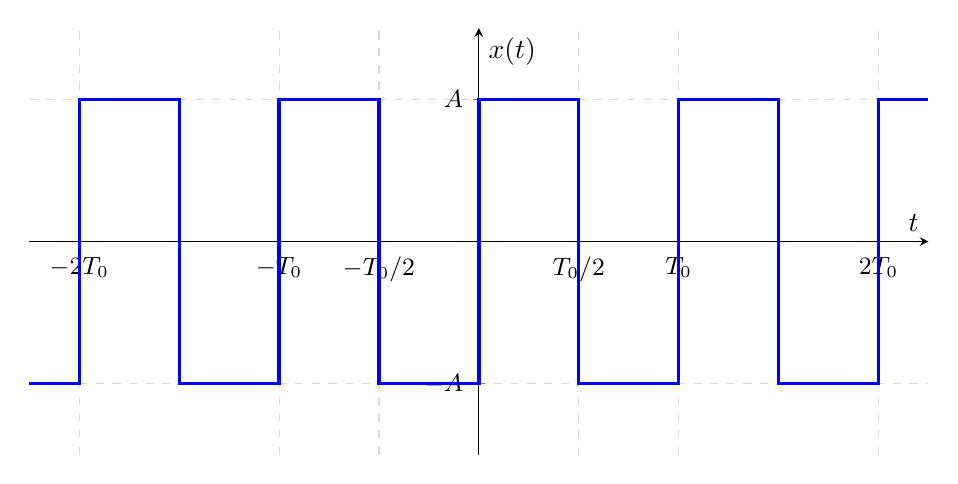
\begin{tikzpicture}
\begin{axis}[
    width=13cm, 
    height=7cm,
    axis lines=middle,
    xlabel={$t$},
    ylabel={$x(t)$},
    xmin=-4.5, 
    xmax=4.5,
    ymin=-1.5, 
    ymax=1.5,
    xtick={-4, -2, -1, 1, 2, 4},
    xticklabels={$-2T_0$, $-T_0$, $-T_0/2$, $T_0/2$, $T_0$, $2T_0$},
    ytick={-1, 1},
    yticklabels={$-A$, $A$},
    grid=both,
    grid style={dashed, gray!30},
    tick label style={font=\small},
    clip=false
]

% Draw the square wave using simple lines
\draw[blue, very thick] 
    (axis cs:-4.5, -1) -- (axis cs:-4, -1) -- (axis cs:-4, 1) -- (axis cs:-3, 1) 
    -- (axis cs:-3, -1) -- (axis cs:-2, -1) -- (axis cs:-2, 1) -- (axis cs:-1, 1)
    -- (axis cs:-1, -1) -- (axis cs:0, -1) -- (axis cs:0, 1) -- (axis cs:1, 1)
    -- (axis cs:1, -1) -- (axis cs:2, -1) -- (axis cs:2, 1) -- (axis cs:3, 1)
    -- (axis cs:3, -1) -- (axis cs:4, -1) -- (axis cs:4, 1) -- (axis cs:4.5, 1);

\end{axis}
\end{tikzpicture}
    \caption{The periodic square wave signal $x(t)$ with odd symmetry.}
\end{figure}

\textbf{Solution:}
$$a_k = \frac{1}{T_0} \int_{T_0} x(t) e^{-jk\omega_0 t} \dd t = \frac{1}{2} \int_{0}^{2} x(t) e^{-jk\pi t} \dd t = \frac{1}{jk\pi} \left[ 1 - (-1)^k \right]$$

For even $k$: $a_k = 0$; For odd $k$: $a_k = \frac{2}{jk\pi}$

\textbf{Answer:} $a_k = \begin{cases} 0 & \text{even } k \\ \frac{2}{jk\pi} & \text{odd } k \end{cases}$
\end{example}

\end{document}